% Document Class is specified here. We're using the Homework Template
\documentclass[12pt, a4paper]{article}

\usepackage{graphicx}
\usepackage{float}
\usepackage{geometry}
\usepackage{verbatim}
\usepackage{listings}

\lstset{
  basicstyle=\itshape,
  xleftmargin=3em,
  literate={->}{$\rightarrow$}{2}
           {ε}{$\epsilon$}{1}
}

\geometry{a4paper, margin=1in}

\title{Week 6 CS-312 Homework}
\author{
	Cory Ness
	\and
	Jack Engledow
	\and
	James Sgrazzutti
}

\begin{document}

\maketitle

\section{Problem 8.2}
\subsection{Question}
Give a regular grammer for $L$ of the form
\begin{lstlisting}
S -> SaS | b
\end{lstlisting}
\subsection{Answer}
\begin{lstlisting}
S -> b | bT
T -> aG
G -> b | bT
\end{lstlisting}

\section{Problem 8.8}
\subsection{Question}
Give a PDA equivalent to the following grammar:
\begin{lstlisting}
S -> aAA
A -> aS | bS | a
\end{lstlisting}
\subsection{Answer}
\begin{center}
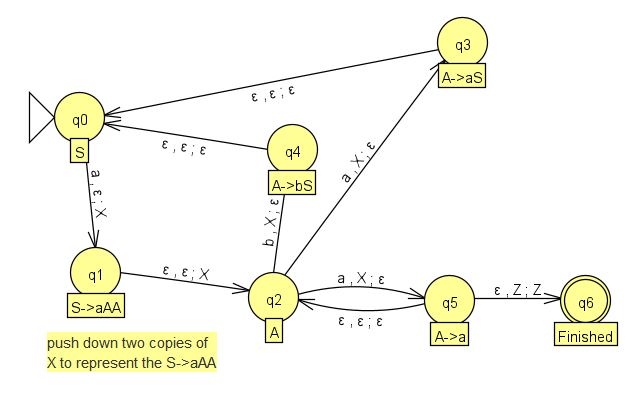
\includegraphics[scale=1]{8.8}
\end{center}

\section{Problem 8.11}
\subsection{Question}
A 2-PDA is like a PDA except that it has two stacks. Show the following can be recognized by a 2-PDA.
\subsection{$\{0^{n}1^{n}2^{n} : n \geq 0 \}$}
\textbf{q0, initial state.} Transitions to itself on $0$ while pushing $X$ to the first stack. Transitions to q1 on nothing.\newline
\textbf{q1.} Transitions to itself on $1$ while popping $X$ from the first stack, pushes $X$ to the second stack. Transitions to q2 on nothing.\newline
\textbf{q2.} Transitions to itself on $2$ while popping $X$ from the second stack. Transitions to q3 on nothing while popping $Z$ from both stacks and pushing $Z$ onto both stacks.\newline
\textbf{q3, final state.}
\subsection{$\{0^{n}1^{n}2^{n}3^{n} : n \geq 0 \}$}
\textbf{q0, initial state.} Transitions to itself on $0$ while pushing $X$ to the first stack. Transitions to q1 on nothing.\newline
\textbf{q1.} Transitions to itself on $1$ while popping $X$ from the first stack, pushes $X$ to the second stack. Transitions to q2 on nothing while popping and pushing $Z$ on the first stack.\newline
\textbf{q2.} Transitions to itself on $2$ while popping $X$ from the second stack and pushing $X$ to the first stack. Transitions to q3 on nothing while popping and pushing $Z$ on the second stack.\newline
\textbf{q3.} Transitions to itself on $3$ while popping $X$ from the first stack. Transitions to q4 on nothing while popping $Z$ from both stacks and pushing $Z$ onto both stacks.\newline
\textbf{q4, final state.}
\subsection{$\{x\#x : x \in \{0,1\}^{*} \}$}
\textbf{q0, initial state.} Transitions to itself on $0$, pushing $0$ to the first stack. Transitions to itself on $1$, pushes 1 to the first stack. Transitions to q1 on $\#$.\newline
\textbf{q1.} Transitions to itself on nothing, popping $0$ from the first stack, and pushing $0$ to the second stack. Transitions to itself on nothing, popping $1$ from the first stack, and pushing $1$ to the second stack. Transitions to q2 on nothing, popping and pushing $Z$ from the first stack.\newline
\textbf{q2.} Transitions to itself on $1$, popping $1$ from the second stack. Transitions to itself on $0$, popping $0$ from the second stack. Transitions to q3 on nothing, popping and pushing $Z$ from both stacks.\newline
\textbf{q3, final state.}

\section{Problem 9.2}
\subsection{Question}
Convert the following grammar with start variable $S$ into Chomsky Normal Form.
\begin{lstlisting}
S -> ASa | aB
A -> B | S
B -> b | ε
\end{lstlisting}
\subsection{Answer}
\begin{lstlisting}
S -> AC | DB
A -> B | S | b | ε
C -> SD
D -> a
\end{lstlisting}

\section{Problem 9.4}
\subsection{Question}
Show that the language $\{a^{n}b^{2n}a^{n}\}$ is not context-free.
\subsection{Answer}
Choose string $z=0^{k}1^{2k}2^{k}$. Split the string into $z=uvwxy$. Because $vwx$ combined has a length of at most $k$, the string $vx$ cannot contain both $0$'s and $2$'s, and contains at least 1 symbol because $vx$ must be nonempty. Therefore, $z^{0}=uwy$ must contain fewer than $1^{2k}$ $1$'s or an uneven number of $0$'s and $2$'s.

\section{Problem 9.12}
\subsection{Question}
Show by example that context-free languages are \textit{not} closed under intersection. Hint: Start with the context-free language $\{0^{n}1^{n}2^{m}\}$.
\subsection{Answer}
Start with $L_{1}$ and $L_{2}$ where $L_{1} = \{0^{n}1^{n}2^{m}\}$ and $L_{2} = \{0^{m}1^{n}2^{n}\}$. Both $L_{1}$ and $L_{2}$ are context-free languages. $L_{1} \cap L_{2} = \{0^{n}1^{n}2^{n}\}$ which is not a context-free language.

\section{Problem 9.17}
\subsection{Question}
A CFG is called linear if the right-hand side of every production contains at most one variable. Thus, a regular grammar is always linear. But a linear grammar need not generate a regular language; for example, we saw that palindromes are generated by a linear grammar. Show that the set of languages generated by linear grammars is closed under union.
\subsection{Answer}
Start with languages $L_{1}$ and $L_{2}$ where both $L_{1}$ and $L_{2}$ are linear. Produce a new language from the union of the two $L$ where $L -> L_{1} | L_{2}$. Clearly $L$ is also linear, as both its productions contain 1 variable, where the variable is a linear CFG.


\end{document}